\documentclass[a4paper]{article}
\usepackage[utf8]{inputenc}
\usepackage{color}
\usepackage{url}
\usepackage[utf8]{inputenc}
\usepackage{graphicx}
\usepackage[english,serbian]{babel}
\usepackage[unicode]{hyperref}
\hypersetup{colorlinks,citecolor=green,filecolor=green,linkcolor=blue,urlcolor=blue}

\begin{document}

\title{Džonatan Bouen\\ \small{Seminarksi rad u okviru kursa\\Tehničko i naučno pisanje\\Matematički fakultet}}

\author{Vladimir Jovanović\\vlad.jov.096@gmail.com \and Katarina Grbović\\kat.grbovic@gmail.com \and Marija Papović\\mpapovic27@gmail.com\and Andrea Mefailovski Stanojević\\andrea.mefst2001@gmail.com}
\date{}
\maketitle

\begin{abstract}
\textbf{Džonatan P. Bouen} (rođen 1956. godine) je britanski stručnjak za računare.
\end{abstract}

\tableofcontents
\newpage

\begin{tabular}{|l|l|}

\hline
\multicolumn{2}{|c|}{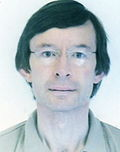
\includegraphics[scale=6]{Jonathan_Bowen_photograph.jpg}} \\
\hline
\textbf{Datum rođenja} & 1956.\\
\hline
\textbf{Mesto rođenja} & Oksford, Ujedinjeno Kraljevstvo\\
\hline
\textbf{Prebivalište} & Oksford\\
\hline
\textbf{Državljanstvo} & Ujedinjeno Kraljevstvo\\
\hline
\textbf{Škola} & Univerzitetski koledž (Oksford)\\
\hline
\multicolumn{2}{|c|}{\textbf{Naučna karijera}} \\
\hline
\textbf{Polje} & Informatika \\ 
& Informaciona tehnologija \\ 
& Muzejska informatika\\
\hline
\textbf{Institucije} & \textit{Museophile Limited}\\
& Univerzitet u Birmingemu\\
& Univerzitet u Redingu\\
& Univerzitet u Oksfordu\\
& \textit{London South Bank} univerzitet\\
& Imperijal Koledž, London\\
\hline
\textbf{Poznat po} & Formalne metode\\
& \textit{Z-notacija}\\
& Stranice muzeja virtuelne biblioteke\\
& Virtuelni muzej računarstva\\
\hline
\textbf{Uticaji} & Dejvid Berman\\
& Džek Kouplend\\
& Majk Gordon\\
& Džejms Hemzli\\
& Toni Hor\\
& Klif Džouns\\
& Alan Tjuring\\
\hline
\textbf{Uticao na} & Majk Hinči\\
& Kevin Lano\\
\hline

\end{tabular}

\newpage
\section{Pregled}
\label{sec:pregled}
Džonatan Bouen je predstavnik „Museophile Limited” kompanije i profesor emeritus na London South Bank univerzitetu, gde je rukovodio Centrom za primenjene formalne metode. Bio je profesor računarske nauke na Univerzitetu u Birmingemu, gostujući profesor na institutu Prat (Njujork), Univerziteta u Vestminsteru, Kings koledža (London), i gostujući akademik na Londonskom univerzitetskom koledžu.

\section{Obrazovanje}
Rođen je u Okfsordu, sin Hamfrija Bouena, a školovao se u tzv. „Dragon School” (Oksford) i u školi u Brajanstonu pre nego što je maturirao na Univerzitetskom koledžu u Oksfordu, gde je stekao zvanje magistra inžinjerskih nauka. 
\section{Karijera}
Bouen je kasnije radio na koledžu „Imperial College” u Londonu, kompjuterskoj laboratoriji univerziteta u Oksfordu (sada odseku za informatičke tehnologije na univerzitetu u Oksfordu), na Univerzitetu u Redingu i univerzitetu „London South Bank”. Njegov rani rad bio je zasnovan generalno na formalnim metodama, a kasnije naročito na „Z-notaciji” (engl. \textit{the Z notations}). Bio je predstavnik grupe „Z-korisnika” (engl. \textit{the Z user group}) od ranih 1990-ih godina do 2011. godine. Proglašen je predstavnikom britanskog kompjuterskog društva „FACS” (engl. \textit{Specialist Group on Formal Aspects of Computing Science}) 2002. godine. Od 2005. godine, Bouen je pomoćnik glavnog urednika novina „Inovacije u sistemu i softverskom inženjerstvu”. Pored toga, saradnik je i urednika naslovne strane novina „ACM Computing Surveys”, pokrivajući oblast softverskog inženjerstva i formalnih metoda. Od 2008.–2009. godine, bio je saradnik u „Praxis High Integrity Systems” i radio na velikom industrijskom projektu koristeći Z-notacije. 

\section{Odabrane knjige}

Izvor \cite{misc:1} se nalazi u tekstu. \\ 
Izvor \cite{misc:2} se nalazi u tekstu. \\
Izvor \cite{misc:3} se nalazi u tekstu.\\
Izvor \cite{misc:4} se nalazi u tekstu.\\
Izvor \cite{misc:5} se nalazi u tekstu.\\
Izvor \cite{misc:6} se nalazi u tekstu.\\
Izvor \cite{misc:7} se nalazi u tekstu.\\
Izvor \cite{misc:8} se nalazi u tekstu.\\
Izvor \cite{misc:9} se nalazi u tekstu.\\
Izvor \cite{book:1} se nalazi u tekstu.\\
Izvor \cite{book:2} se nalazi u tekstu.\\
Izvor \cite{aritcle:1} se nalazi u tekstu.\\
Izvor \cite{article:2} se nalazi u tekstu.\\
Izvor \cite{article:3} se nalazi u tekstu.\\
Izvor \cite{article:4} se nalazi u tekstu.\\

\bibliography{notes} 
\bibliographystyle{ieeetr}

\begin{itemize}
\item Bouen, Dž.P., urednik, Towards Verified Systems. Elsevier, Real-Time {\itshape Safety Critical Systems series}, tom 2, 1994. ISBN 0-444-89901-4
\item Hinči, M.G. i Bouen, Dž.P., urednici {\itshape Applications of Formal Methods}. Prentice Hall International Series in Computer Science, 1995. ISBN 0-13-366949-1.
\item Bouen, Dž.P., {/itshapem Formal Specification and Documentation using Z: A Case Study Approach }. International Thomson Computer Press, International Thomson Publishing, 1996. 
\item Bouen, Dž.P. i Hinči, M.G., urednici,{\itshape High-Integrity System Specification and Design. }Springer-Verlag , London, 1999. ISBN 3-540-76226-4.
\item Hinči, M.G. i Bouen, Dž.P., urednici,{\itshape Industrial-Strength Formal Methods in Practice. } Springer-Verlag, London, 1999. ISBN 1-85233-640-4.
\item Hierons, R., Bouen, Dž.P., i Harman, M., urednici,{\itshape  Formal Methods and Testing} . Springer-Verlag, LNCS, tom 4949, 2008. ISBN 978-3-540-78916-1.
\item Berger, E., Batler, M., Bouen, Dž.P., i Boka, P., urednici, {\itshape Abstract State Machines, B i Z }. Springer-Verlag, LNCS, tom 5238, 2008. ISBN 978-3-540-87602-1.
\item Boka, P., Bouen, Dž.P., i Sidiki, Dž.I., urednici,{\itshape Formal Methods: State of the Art and New Directions}. Springer, 2010. ISBN 978-1-84882-735-6, e-ISBN 978-1-84882-736-3, doi:10.1007/978-1-84882-736-3.
\item Bouen, Dž.P., Kin, S., i Ng, K., urednici,{\itshape Electronic Visualisation in Arts and Culture} . Springer Series on Cultural Computing, Springer, 2013. ISBN 978-1-4471-5406-8.
\item Kouplend, Dž., Bouen, Dž.P., Sprevak, M., Vilson, R., i dr., The Turing Guide. Oxford University Press, 2017. ISBN 978-0198747826, ISBN 978-0198747833.
\item Kouplend, Dž., Bouen, Dž.P., Sprevak, M., Vilson, R., i dr., The Turing Guide. Oxford University Press, 2017. ISBN 978-0198747826, ISBN 978-0198747833.
\item Hinči, M.G., Bouen, Dž.P., Olderog, E.-R., urednici,{\itshape Provably Correct Systems}. Springer International Publishing, NASA Monographs in Systems and Software Engineering series, 2017. ISBN 978-3-319-48627-7, doi:10.1007/978-3-319-48628-4.
\item Đanini, T. i Bouen, Dž.P., urednici,{\itshape Museums and Digital Culture: New Perspectives and Research}. Springer Series on Cultural Computing, Springer, 2019. ISBN 978-3-319-97456-9, e-ISBN 978-3-319-97457-6, doi:10.1007/978-3-319-97457-6
\end{itemize}

\section{Reference}

\begin{itemize}

\item Bouen, Džonatan Piter: Who's Who in the World, Marqius Who's Who, 18. izdanje, 2001.
\item H-museum information
\item Museums and the Web conference information
\item "Film on the Web conference information"
\item International Center for Scientific Research information
\end{itemize}

\section{Spoljašnje veze}

\begin{itemize}

\item Lični sajt
\item Početna stranica na sajtu Saut Benk univerziteta u Londonu (engl. London South Bank University)
\item Džonatan Bouen na DBLP serveru za bibliografiju
\item Džonatan Bouen čije je publikacije indeksirao Gugl akademik (engl. Google Scholar)
\item Džonatan Bouen na pretraživaču Majkrosoft akademik (engl. Microsoft Academic)
\item Džonatan Bouen u bazi podataka projekat Matematička genealogija (engl. Mathematics Genealogy Project)
\end{itemize}


\end{document}
